\documentclass[12pt, final]{article}
\usepackage[margin= 0.75in]{geometry}
\usepackage{amsfonts}
\usepackage{amsthm}
\usepackage{amsmath}
\usepackage{mathabx}
\usepackage{ulem}
\usepackage{enumerate}
\usepackage{float}
\usepackage{graphicx}
\graphicspath{{../Code/PLOTS/}}
\usepackage{color}
\usepackage{subfigure}
\usepackage{commath}
\usepackage[font = scriptsize]{caption}

\begin{document}

\newcommand{\Pois}{\text{Pois}}

\newtheorem{prop}{Proposition}


\title{Think of a title later}
\author{Ansel Blumers and Ankan Ganguly}
\maketitle

\begin{abstract}
Abstract goes here.
\end{abstract}

\newpage

\tableofcontents

\newpage

\section{Introduction}

Write an introduction here.

\section{Methods}

In this paper, we used the simulated Integrate and Burst model introduced in \cite{Fiete}. We then implemented STDP learning and Hebbian learning.

\subsection{Integrate and Burst Model}

Our integrate and burst model is an implementation of equations described in \cite{Fiete}. For convenience, we also provide a detailed description of these equations here. There are \(N\) neurons connected in an all-to-all environment. Each neuron \(i\) bursts when its membrane potential, \(V_i\), hits the threshold \(V_\theta\). We assume that every neuron bursts for \(T_{burst}\) time. While bursting, each neuron fires four times uniformly over the burst interval before resetting to \(V_{reset}\).

When a neuron is not bursting, its potential is governed by a typical conductance based leaky integrate and fire model with built-in inhibition:

\begin{equation}
\tau_V \od{V_i}{t} = -g^L(V - V^L) - g^E_i(V - V^E) - g^I_i(V - V^I)
\label{Potential}
\end{equation}

The leak conductance, \(g^L\), is assumed to be a homogeneous constant input, as is the leak potential \(V^L\). Notice that in the absence of excitatory or inhibitory conductance, neuron \(i\) will tend to \(V^L\). Therefore we can say that the leak potential is also equal to the rest potential.

The excitation potential, \(V^E\), and the inhibition potential, \(V^I\), act as upper and lower bounds on untethered \textcolor{red}{(What was the word for IF potential plots without a firing threshold?)} potential respectively. 

The excitation conductance, \(g^L\), is defined by the activity in neighboring neurons as well by external random stimulation:

\[g^L = Ws + W_0b\]

Where \(W_{ij}\) is the strength of the synapse from neuron \(j\) to neuron \(i\), \(W_0\) is the conductance strength of external synapses and \(b\) is a Poisson random variable with frequency \(r_{in}\). \(s_i\) is the activation of neuron \(i\). It is incremented each time neuron \(i\) fires, and it decays by

\[\od{s}{t} = -\tau s\]

The inhibitory conductance, \(g^I\), is defined as the sum of the adaptation inhibition, \(g^I_{ada}\), and the global inhibition, \(g^I_{glob}\). The adaptation inhibition is the internal inhibition generated by activation of a neuron. It is defined by the same equations as \(s_i\), but with a constant multiplier \(A_a\) and a slower time-constant \(\tau_{ada}\).

\subsection{Learning}

The purpose of this paper is to replicate and test some of the claims made in \cite{Fiete}. One of the claims made is that the model used by \cite{Fiete} demonstrates how STDP can contribute to the synchronous regular synfiring chains exhibited in Zebra Finch \textcolor{red}{(Where? Maybe cite second paper here?)}. 

\subsubsection{STDP Learning}

We followed \cite{Fiete} in our implementation of Learning. Define

\[K(t) = 
\begin{cases}
e^{-t/\tau_{STDP}} &\text{ if } t \neq 0\\
0 &\text{ otherwise}
\end{cases}
\]

as the STDP kernel. Let \(\rho(t) = \sum_{k} \delta(t - t_k)\)

\subsubsection{Hebbian Learning}

Talk about Hebbian learning here.

\subsection{Parameter Choices}

Talk about how we chose parameters here.

\section{Results}

Introduce the big idea and what we got.

\subsection{Parameter Tuning}

\begin{itemize}
\item 4000 Hz doesn't work! (Burst Plot)

\item Mention annealing and our choice of \(r_{in}, \eta\) and \(\epsilon\). Name the two data sets we refer to for the remainder of the paper. (Scatter Error Function)

\item Setting \(w_{max}\). (Burst History)
\end{itemize}

\subsection{Convergence and Stability}

\begin{itemize}
\item Demonstrate the stability of our IB model by showing the firing rate plot and how it splits according to \(r_{in}\).

\begin{figure}[H]
\centering
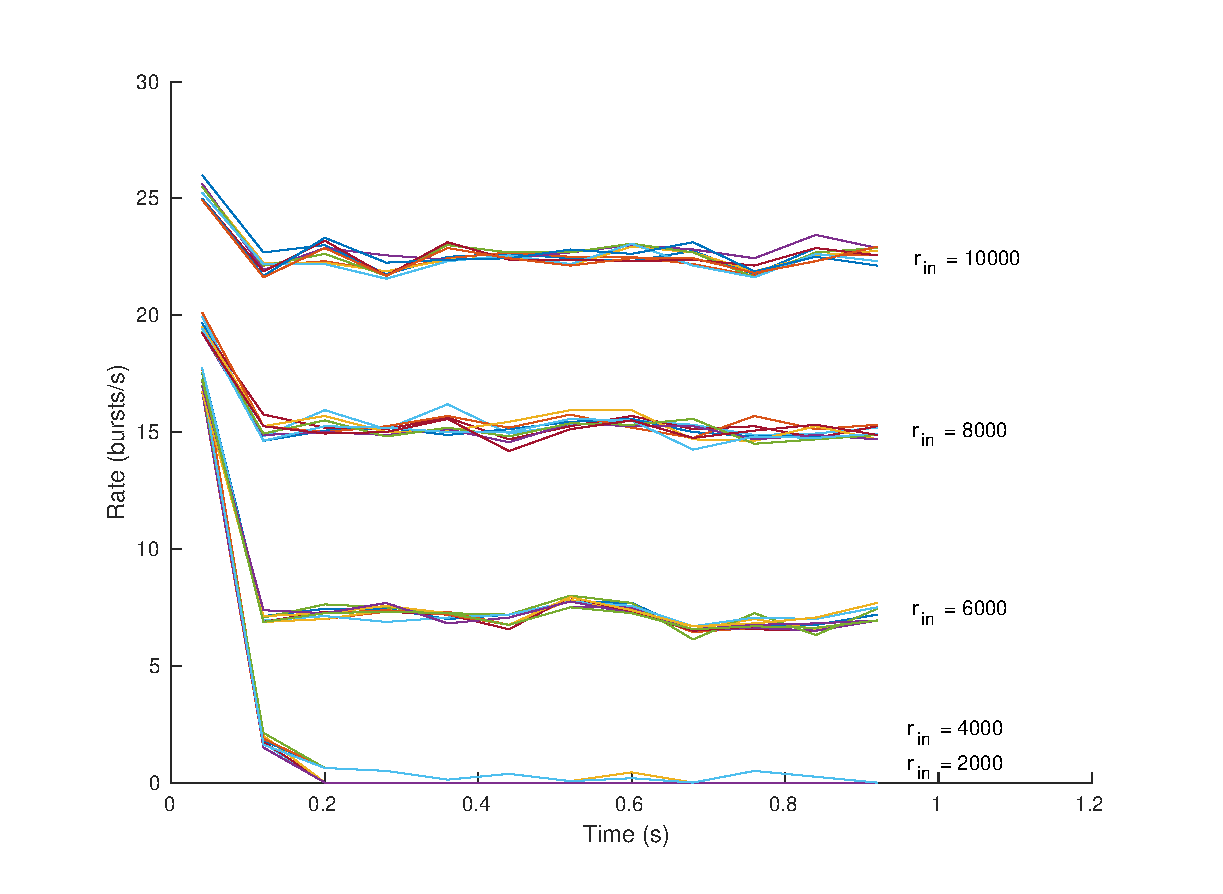
\includegraphics[scale = 0.4]{Firing_Rate_Binsize_80ms.eps}
\label{FR}
\caption{Caption will go here}
\end{figure}

\item Plot Weight and \(WW^T\) for 4000 and 6000 Hz to show some level of convergence.

\item Plot error function over time from normal and from permutation matrix

\item Describe why the error function converges away from 0.
\end{itemize}

\subsection{Hebbian Learning versus STDP}

\begin{itemize}
\item Introduce the idea of the refutation. 
\item Give a theoretical description why the type of learning should be relatively unimportant.
\item Compare plots (\(WW^T\), Error vs Time, Burst History).
\end{itemize}

\section{Discussion}

Further improvements that could be made to our model and where this research could be taken.

\section{Summary}

Quick summary of our results and everything.



\bibliographystyle{plain}
\bibliography{Songbird_paper}

\end{document}